\documentclass{article}
\usepackage[utf8]{inputenc}
\usepackage{amssymb}
\usepackage{amsmath}
\usepackage{graphicx}
\usepackage{fullpage}
\usepackage{titlesec}
\usepackage{multirow}
\titleformat{\section}{\bfseries}{\thesection}{1em}{}
\titleformat{\subsection}{}{\thesection}{1em}{}
\usepackage{tikz}
\usetikzlibrary{positioning}
\usepackage{listings}
\usepackage{color}
\usepackage{lineno}
\renewcommand\linenumberfont{\normalfont\small\sffamily}


\begin{document}

\section*{Results}

\paragraph{}
We investigated the relationship between entropy and cache traces, attempting to relate it to the cachability or prefetchability of a given trace.  What we found across several real-world traces is that distinct items are repeated very few times, making them poor predictors of what would be accessed next.  However, the differences between consecutive accesses (strides) are much more predictable.  While this predictability doesn't indicate that a trace will perform better in a cache on its own, it does indicate that a cache running the trace would greatly benefit from a prefetcher that can use stride data to predict the next access.

The predictability of the strides is evident in both the distribution of strides overall and by using conditional entropy measurements.  On any of the traces we tested, the distribution of strides is heavy-headed, leading to a lower entropy value than if the distribution was uniform.  This difference is consistently 2-5 bits of entropy for traces of all sizes (on the order of 1000-1000000 accesses) (Fig. \ref{fig:expected}).

\begin{figure}[ht]
    \centering
    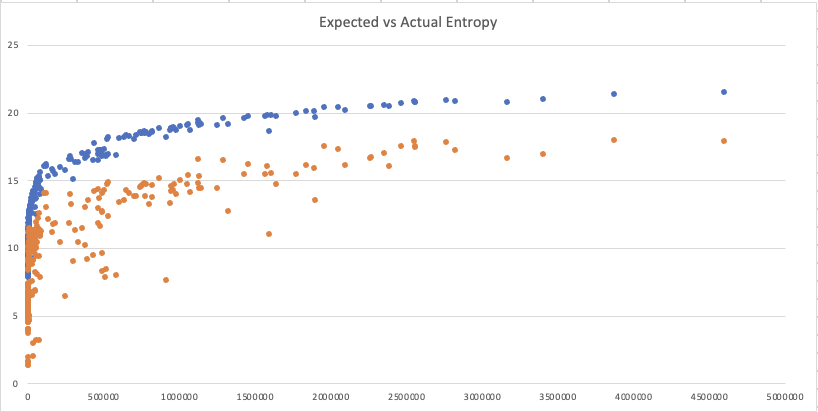
\includegraphics{expected entropy.png}
    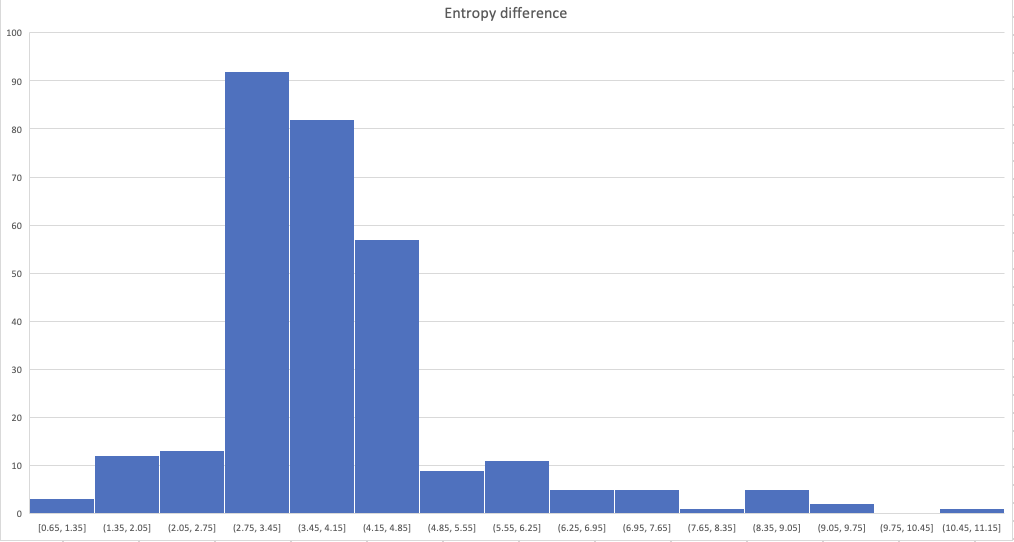
\includegraphics[scale=0.8]{entropy diff.png}
    \caption{Expected entropy (blue) and actual entropy (orange) plotted against trace length, and a histogram of the differences.  Expected entropy is calculated as the entropy if the strides are uniformly distributed.}
    \label{fig:expected}
\end{figure}
\newpage

We also measured the entropy of the strides conditioned on knowing the last $N$ strides to see how predictable the traces are within a small window.  When $N = 1$, the conditional entropy stayed consistently below 5 bits, with an average of 2.37 bits, indicating a high degree of predictability (Fig.\ref{fig:cond1}).  As $N$ increases, the entropy falls off quickly, in part due to a lack of sample size.  For $N = 2$, most traces have entropy below 1.5 bits, with the average being about 0.7 bits (Fig.\ref{fig:cond2}).  Higher values of $N$ offer very little improvement to this value, and the conditions are repeated so rarely at $N = 3$ or higher that the entropy is measured as close to 0 due to a lack of samples.  However, the sample size for $N = 2$ may be large enough to conclude that it offers significant improvement over $N = 1$.

\begin{figure}[ht]
    \centering
    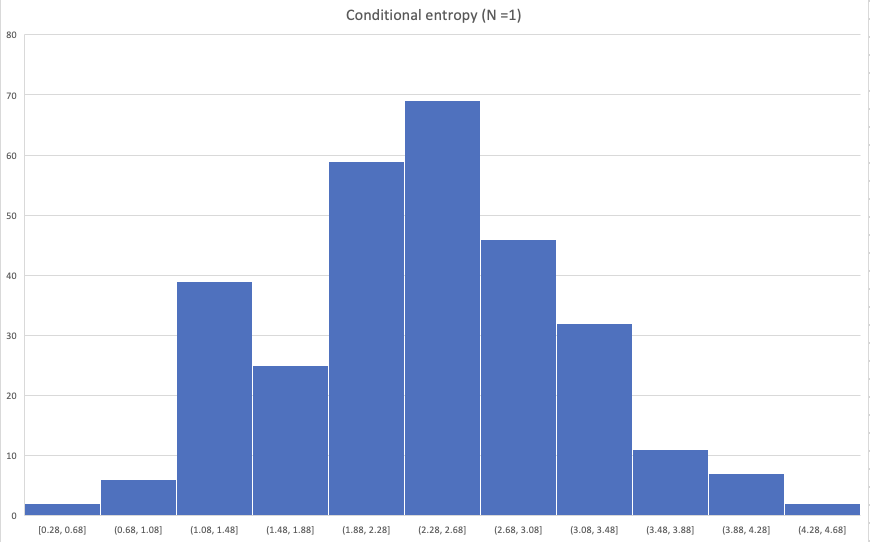
\includegraphics[scale=0.7]{conditional 1.png}
    \caption{Histogram of the conditional entropy when $N = 1$}
    \label{fig:cond1}
\end{figure}

\begin{figure}[ht]
    \centering
    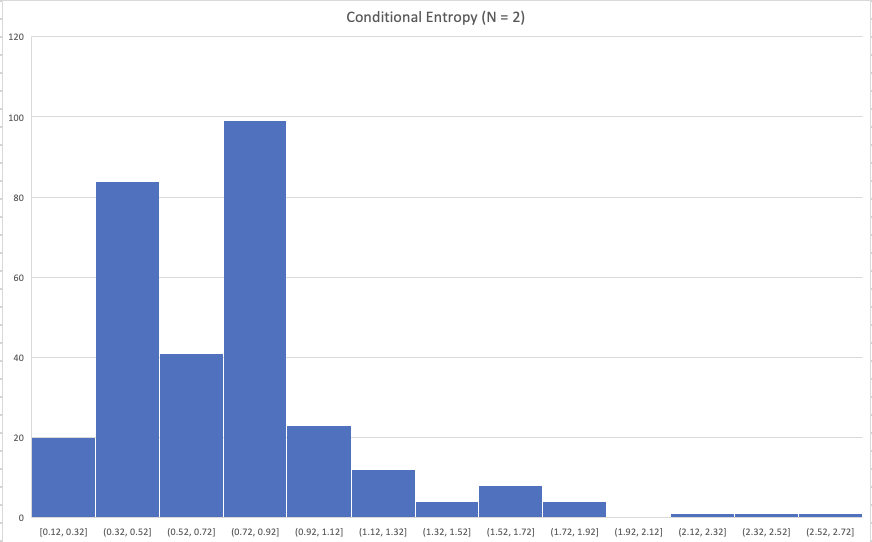
\includegraphics[scale=0.7]{conditional 2.png}
    \caption{Histogram of the conditional entropy when $N = 1$}
    \label{fig:cond2}
\end{figure}

These results indicate that it could be worthwhile to give a prefetcher the resources to keep track of strides conditioned on the last 2 that have been seen, at least in longer traces.  The predictability of the strides based on only the previous stride can also provides large benefits to any prefetcher.  Caches without prefetchers likely cannot take advantage of stride patterns without large amounts of resources, so these entropy values do not mean much for the cachability of a trace.

\end{document}
